\documentclass[review,a4paper,fleqn]{cas-sc}
\usepackage{amsmath,amssymb}
\usepackage{booktabs,tabularx,array,longtable}
\usepackage{graphicx,float,pdflscape}
\usepackage{siunitx}
\usepackage{url}
\hypersetup{hidelinks}
\usepackage{fontspec}
\defaultfontfeatures{Ligatures=TeX}
\setmainfont{Times New Roman}
\setsansfont{Times New Roman}
\setmonofont{Times New Roman}
\newcommand{\mminus}{\mathbin{\text{\char"2212}}}
\newcommand{\mplusminus}{\mathbin{\text{\char"00B1}}}
\setlength{\emergencystretch}{3em}
\newcommand{\cotwo}{CO\textsubscript{2}}
\newcommand{\cotwoe}{CO\textsubscript{2}e}
\newcommand{\chfour}{CH\textsubscript{4}}
\newcommand{\ntwoo}{N\textsubscript{2}O}
\begin{document}
\shorttitle{OpenDC-LCA for data center decisions}
\shortauthors{Stevens et al.}
\title[mode=title]{OpenDC-LCA: An open-source framework for applying published data center cooling LCAs to facility decisions}
\author[uark,hfa]{Braden Stevens}
\author[uark,hfa]{Pengjiang Xiang}
\author[ahpcc]{Pawel Wolinski}
\author[its]{Charles Dwyer}
\author[ornl]{Yimin Chen}
\author[uark]{Darin Nutter}
\author[uark]{Han Hu}[orcid=0000-0002-9667-1698]
\cormark[1]
\ead{hanhu@uark.edu}
\affiliation[uark]{organization={Department of Mechanical Engineering, University of Arkansas}, city={Fayetteville}, state={AR}, postcode={72701}, country={U.S.}}
\affiliation[ahpcc]{organization={Arkansas High Performance Computing Center, University of Arkansas}, city={Fayetteville}, state={AR}, postcode={72701}, country={U.S.}}
\affiliation[its]{organization={IT Services, University of Arkansas}, city={Fayetteville}, state={AR}, postcode={72701}, country={U.S.}}
\affiliation[ornl]{organization={Building Technologies Research and Integration Center, Oak Ridge National Laboratory}, city={Oak Ridge}, state={TN}, postcode={37830}, country={U.S.}}
\affiliation[hfa]{organization={Harrison French \& Associates Ltd.}, city={Bentonville}, state={AR}, postcode={72712}, country={U.S.}}
\cortext[1]{Corresponding author}
\begin{abstract}
Data center modernization changes computing capacity, heat rejection, electricity use, and equipment replacement together. A cooling comparison can guide a facility decision only when its service definition, life cycle method, and physical scope apply to the proposed installation. This paper develops OpenDC-LCA, an open-source framework that traces the evidence needed for that judgment. The Microsoft/WSP comparison of air, cold-plate, single-phase immersion, and two-phase immersion cooling provides the case study. Arithmetic reconstruction matched 24 released totals, while the released electricity information did not resolve the stated AR5 100-year global-warming-potential basis. Nine annual U.S. eGRID datasets, recalculated on an AR5 basis, showed a 32.46\% decline in the national direct-generation factor from 2012 to 2023. Those data provide electricity context without replacing the life cycle electricity model in the cooling comparison. A deterministic worst-case certificate found that the nominal first-ranked architecture reversed when all declared assumption blocks moved adversely by an equal half-width of 1.32\%. Comparable computing service, time-aligned use-phase demand, and architecture-resolved equipment quantities are the immediate evidence needs for a facility-specific assessment. The resulting workflow makes the numerical basis, its applicable range, and the missing evidence visible before a cooling technology is selected.

\end{abstract}
\begin{keywords}
data center \sep life cycle assessment \sep energy efficiency \sep lifecycle electricity \sep functional equivalence \sep sensitivity analysis \sep open-source software
\end{keywords}
\maketitle

\section{Introduction}
\subsection{Cooling-system lifecycle context}
Data center modernization couples rapidly changing computing hardware to long-lived electrical and cooling infrastructure. Facility managers must therefore evaluate computing capacity together with thermal management and environmental burden \cite{ref1,ref2}. At the equipment level, increasing processor heat flux and rack density are moving many facilities from room-air cooling toward rear-door heat exchangers, direct-to-chip cold plates, and single- or two-phase immersion \cite{ref3,ref4,ref5}. A useful assessment must connect a proposed technology change to the corresponding facility-wide consequences.

Cooling architecture changes the heat-rejection path and the supporting equipment required to operate it. Server fans, pumps, coolant distribution units, heat-rejection temperature, fluid inventory, rack or tank construction, packing density, repair procedures, and achievable clock rate can all change with the cooling approach. System experiments have reported load-dependent differences in coefficient of performance and cost for single- and two-phase immersion \cite{ref6}. Recent single-phase tests show that flow direction, coolant viscosity, and water temperature affect chip temperature, thermal resistance, and power usage effectiveness (PUE) \cite{ref7}. Two-phase experiments likewise show that boiling, pressure stability, and condenser performance require evaluation at server and system levels \cite{ref8}. Equal rack count, equal IT electricity, and equal nameplate capacity can therefore correspond to different computing services.

PUE remains useful for facility energy management. A cooling decision also requires information about equipment production, cooling-fluid loss, replacement, water use, and the computing service delivered. These connected effects motivate a transparent assessment method that identifies both the available evidence and the information needed before a facility adopts a cooling change.

\subsection{Data center LCA literature}
Early environmental assessments showed that operating electricity dominates many data center footprints and that PUE alone can transfer burdens outside the measured facility boundary \cite{ref9}. U.S. studies subsequently linked data centers to spatially varying electricity and water burdens \cite{ref10,ref11}. At the product scale, Isler-Kaya and Karaosmanoglu collected manufacturing inventory for a cooling device and evaluated electricity and waste scenarios \cite{ref12}. Wenzel and Radgen compared energy, material-flow, exergy, and lifecycle assessment methods for a wet cooling tower, illustrating that method choice changes the question answered \cite{ref13}.

Alissa et al. published the most detailed public hyperscale comparison of air, cold-plate, single-phase immersion, and two-phase immersion \cite{ref14}. Their cradle-to-grave model included buildings, support equipment, servers, racks or tanks, cables, cooling fluids, use-phase electricity and water, replacement, and end of life. The use of Vcore-year as the functional unit was a major advance because it allowed packing density and cooling-enabled computation to enter the comparison. The accompanying archive includes normalized contributions, equations, uncertainty material, and a pedigree assessment \cite{ref15}. It does not, however, disclose every licensed background process, architecture-specific bill of quantities, or a transferable mapping from electricity to workload performance.

Recent work has moved closer to architecture- and service-level assessment. d'Orgeval et al. modeled complete data center configurations and reported performance-normalized results for GPU-based subsets \cite{ref16}. Wu et al. released and validated a cooling-plant virtual testbed against three months of operating data, with 7.62\% mean absolute percentage error for power \cite{ref17}. These studies provide performance and architecture evidence that a secondary normalized table cannot supply. ITU-T L.1410 likewise treats the functional unit and the rules for comparative ICT analysis as explicit study choices \cite{ref18}.

Existing data center LCA studies demonstrate the importance of both electricity supply and cooling efficiency, while manufacturer and ICT studies report wide variation in embodied server impacts \cite{ref19,ref20,ref21}. These studies provide valuable inputs for cooling decisions. Their results require additional scrutiny when a facility applies them under a different electricity system, cooling load, or computing-service definition. The remaining gap is a reproducible method for determining whether the evidence supporting a published comparison remains applicable to a new decision context.

\subsection{Temporal and geographic electricity accounting}
Electricity is not a scalar independent of method. Attributional LCA usually requires a consumption mix with upstream generation, transmission, and other indirect processes, whereas eGRID state total-output rates describe direct emissions from in-state generation. Location-based, market-based, and marginal factors answer different questions. Combining location- and market-based accounting inconsistently can double count renewable attributes \cite{ref22,ref23}. Average rates can also fail to represent the effect of workload shifting. Dandres et al. found that average and marginal electricity signals can lead to different real-time data center decisions \cite{ref24}.

Time affects i) cooling performance across load and weather, ii) hourly and long-term grid composition, iii) discrete equipment replacement, and iv) background technology. Dynamic-LCA reviews address temporal inventory, characterization, and prospective background change as separate modeling choices \cite{ref25,ref26}. Open tools such as Temporalis and, more recently, bw\_timex show how temporal information can be propagated through process networks \cite{ref27,ref28,ref29}. For cooling, hourly operation is necessary but insufficient. The grid method, geography, and upstream boundary must also be aligned. A weather file cannot repair an incompatible electricity inventory.

\subsection{Data quality, uncertainty, and decision value}
LCA uncertainty arises from parameters, scenarios, model form, allocation, system boundary, and incomplete knowledge. Monte Carlo propagation is useful when distributions and correlations are supportable. It becomes misleading when arbitrary ranges are presented as confidence. Correlation can materially change propagated uncertainty and cannot be inferred from marginal ranges alone \cite{ref30}. Reviews recommend separating variability from uncertainty and using sensitivity analysis to identify influential assumptions \cite{ref31}. Pedigree matrices can communicate reliability, temporal, geographic, and technological representativeness, but the conversion from qualitative scores to uncertainty is itself a modeling choice \cite{ref32,ref33}.

EPA guidance treats reproducible documentation at flow and process levels as part of data-quality assessment \cite{ref33}. Value-of-information methods prioritize data whose resolution is expected to change a decision instead of improving every weak input indiscriminately \cite{ref34}. For electronics-cooling laboratories, a small PUE difference can decide between nearly tied lifecycle alternatives even when another parameter has poorer pedigree but little decision leverage.

ISO 14040 and ISO 14044 define the LCA framework and requirements, whereas ISO 14071 (2024) specifies the critical-review process and reviewer competencies needed for stronger claims, with particular relevance to comparative assertions intended for public disclosure \cite{ref35,ref36}. Code tests, data checks, and coauthor review can strengthen traceability, but none is a substitute for an independent critical review.

\subsection{Research gap and contributions}
General engines such as openLCA and Brightway calculate process networks and life cycle impacts \cite{ref37,ref38}. Cooling-plant models calculate operational power and thermal performance \cite{ref17}. A facility manager still needs to know whether a published cooling comparison uses a compatible service basis, electricity model, and physical inventory before applying its ranking to a new project. This question connects cooling engineering with life cycle assessment and motivates the analysis presented here.

The Microsoft/WSP comparison provides a public case study of evidence transfer from a published cooling LCA to a proposed facility. The analysis reconstructs the published totals, audits the climate-impact information in the released numerical model, recalculates historical eGRID generation factors on a common climate basis, and calculates partial linked electricity systems from Federal LCA Commons. Declared changes in electricity, use phase, embodied burden, and computing service then test the numerical rank. The accompanying software applies the same metadata requirements to a proposed comparison and reports its sources, calculations, and unresolved evidence gaps. The case study identifies the evidence required before a published cooling comparison can be used in a facility decision.

\section{Framework and methods}
\subsection{Evidence-to-decision framework}
Figure 1 illustrates the OpenDC-LCA architecture from published evidence to a facility decision. The framework begins with the proposed computing service and then compares the life cycle method, electricity scope, and operating conditions with the facility context. When a material evidence gap remains, the framework identifies the measurements or inventories needed for a facility-specific assessment. The repository retains source identifiers, file checksums, field definitions, units, boundaries, and numerical roles for audit. The automated checks characterize available evidence. Source authentication, physical-model validation, and independent critical review remain human tasks.

\begin{figure}
\centering
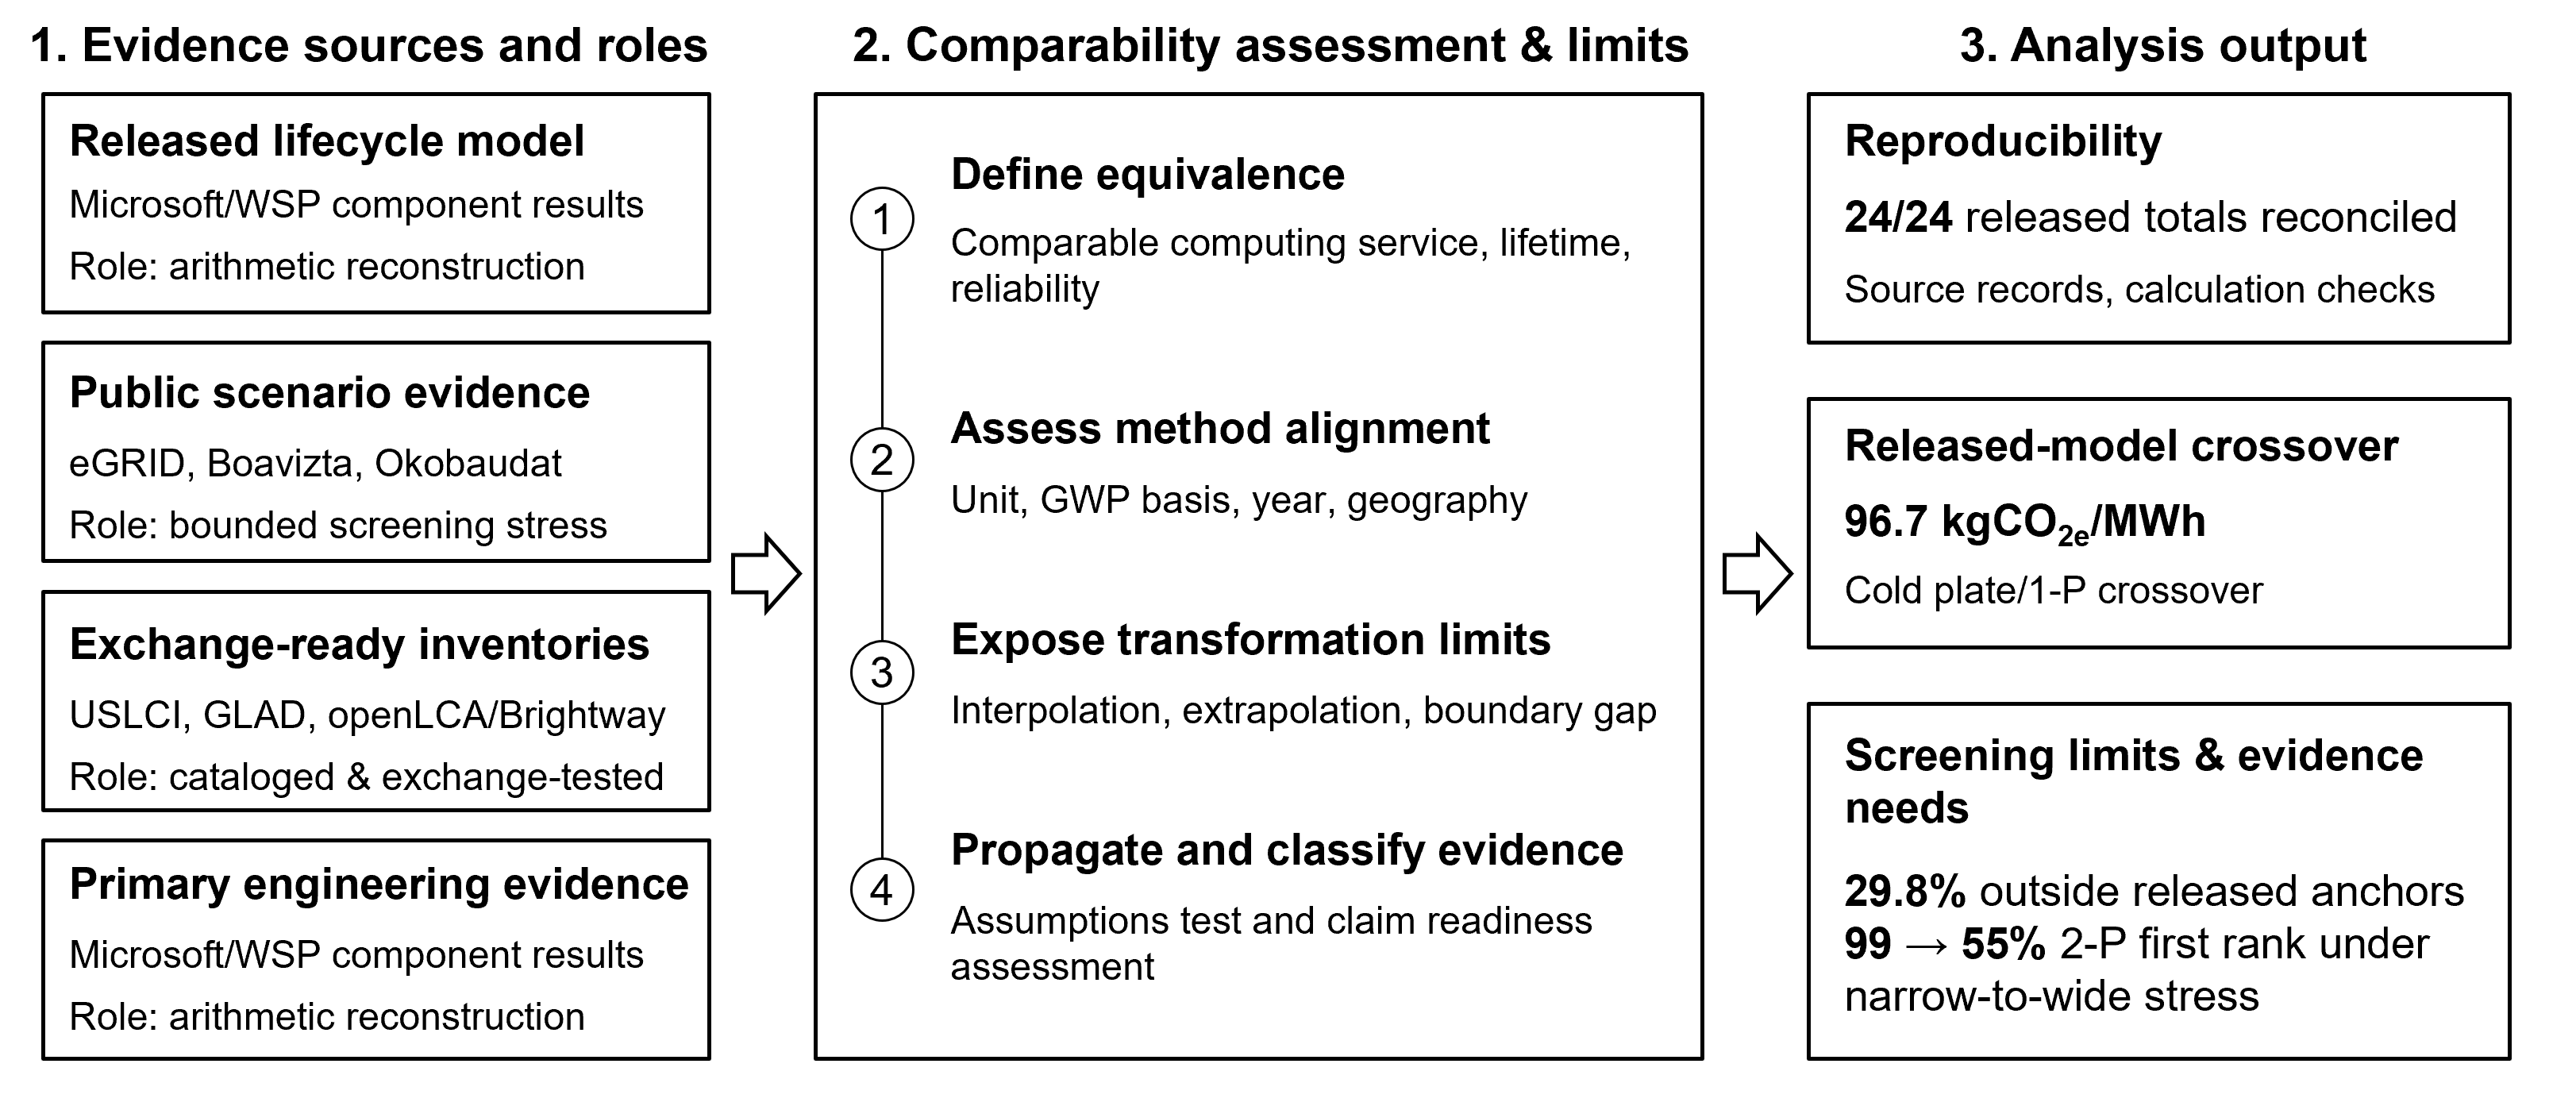
\includegraphics[width=0.98\linewidth]{Figure_1_OpenDC-LCA.png}
\caption{OpenDC-LCA workflow linking a released data center cooling comparison with public electricity data, life cycle inventories, and engineering evidence. The workflow contains a decision context, evidence evaluation, compatibility check, and output stage. The output boxes display the released-total reconstruction count, numerical crossover intensity, state-year rates outside the released electricity anchors, and rank frequencies from the specified stress analysis.}
\label{fig:figure0-opendc-lca-workflow}
\end{figure}

OpenDC-LCA is implemented in Python 3.10 or later and distributed under the MIT License \cite{ref39}. The development branch evaluated here extends version 1.1.0 with interfaces for scenarios, performance maps, reliability and replacement models, openLCA JSON-LD and Brightway mappings, evidence audits, and reports. Before calculation, the comparison validator requires cross-scenario metadata and field-level source mappings. Declared source accuracy, uncertainty-model adequacy, and review status require independent assessment. All interfaces call the same calculation engine.

\subsection{Goal, functional units, and system boundaries}
The practitioner package defaults to one MWh delivered to IT equipment (\texttt{it\_mwh}) for operational screening. That unit is valid for comparison only when alternatives provide equivalent computational output, utilization, quality of service, reliability, and hardware life. The Microsoft/WSP secondary analysis remains in its released functional unit of one Vcore-year. No conversion between IT MWh and Vcore-year was made because the public archive does not provide a workload-independent mapping between them.

The package supports a cooling-system cradle-to-grave boundary and a broader facility cradle-to-grave boundary. The former includes cooling and heat-rejection equipment, fluids, represented maintenance and replacement, operation, and end of life. The latter can also include building, electrical, and IT assets. Common systems may be excluded only when their quantity, performance, lifetime, and end-of-life treatment are unchanged. Onsite water and electricity-supply-chain water are reported separately. Location- and market-based electricity are not merged.

The Open Compute Project (OCP) cloud-provider guideline identifies the same classes of foreground information for data center LCAs, including IT and support equipment, building and electrical infrastructure, operation, cooling water, and end of life \cite{ref50,ref51,ref52}. Its example service denominator should not be substituted for the present operational denominator. The public cooling archive does not provide a workload-independent mapping between a virtual-machine service and delivered IT electricity, and no job-level data are available for the four cooling architectures.

For a liquid-cooled site, the facility water system (FWS) and the technology cooling system (TCS) are separate physical loops when a coolant distribution unit (CDU) transfers heat across its heat exchanger. The TCS includes the CDU-to-rack loop, manifolds, rack equipment, and its coolant. A direct facility connection has no CDU separation and must identify the actual heat-exchange location. This nomenclature specifies the inventory and telemetry information needed for a future site assessment. It makes no inference about the topology or operation of the university site \cite{ref53,ref54,ref55,ref56}.

Operational validation uses a separate measurement boundary. The IT boundary must be metered, and every support-energy item must be classified as metered, allocated, or excluded. A facility PUE requires all support energy within the declared facility boundary. A smaller UPS and dedicated-cooling boundary can report a dedicated-support ratio. The repository measurement protocol specifies the electrical, thermal, workload, calibration, and provenance information needed at a shared-infrastructure site. A common workload is also required before the service denominator can be compared across cooling architectures.

\subsection{Dataset roles and inclusion criteria}
Table 1 identifies the source families used in the analysis and the role each source plays in the resulting claims. The table also states the boundary or data limitation that prevents each source from supporting a broader conclusion. This mapping keeps a readable file, a calculated value, and a decision-ready input from being treated as equivalent forms of evidence.

{\footnotesize
\setlength{\tabcolsep}{3pt}
\begin{longtable}{>{\raggedright\arraybackslash}p{0.18\textwidth}>{\raggedright\arraybackslash}p{0.23\textwidth}>{\raggedright\arraybackslash}p{0.34\textwidth}>{\raggedright\arraybackslash}p{0.16\textwidth}}
\caption{Numerical role and boundary assigned to downloaded evidence.}\\
\toprule
Source and evidence used & Numerical role in this paper & Boundary or transfer limit & Claim class \\
\midrule
\endfirsthead
\caption[]{Numerical role and boundary assigned to downloaded evidence. (continued)}\\
\toprule
Source and evidence used & Numerical role in this paper & Boundary or transfer limit & Claim class \\
\midrule
\endhead
\midrule
\multicolumn{4}{r}{Continued on next page}\\
\endfoot
\bottomrule
\endlastfoot
Microsoft/\allowbreak{}WSP archive with 24 totals, component tables, 2 electricity anchors, and pedigree entries \cite{ref14,ref15} & Arithmetic reconstruction, foreground contribution model, crossover and stress analyses & Licensed background inventories and complete bills of quantities are not public & Released/\allowbreak{}reconstructed \\
\addlinespace[2pt]
EPA eGRID with 459 state/\allowbreak{}DC-\allowbreak{}year rows and 9 U.S. aggregates \cite{ref40,ref41} & Common-\allowbreak{}basis generation-\allowbreak{}rate scenarios and historical trend & Direct generation rates are not consumption-\allowbreak{}based lifecycle electricity inventories & Screening transformation \\
\addlinespace[2pt]
Federal LCA Commons U.S. Electricity Baseline 2023 and IPCC GWP method \cite{ref42} & Linked consumption-\allowbreak{}system factors for 60 balancing authorities, 10 FERC regions, and the United States & Unlinked technosphere inputs remain zero-\allowbreak{}burden cutoffs and are not harmonized with the released cooling foreground & Partial linked-\allowbreak{}system screen \\
\addlinespace[2pt]
Boavizta with 48 server PCF entries \cite{ref43} & Server-\allowbreak{}manufacturing dispersion and common-\allowbreak{}scaling stress & Products, configurations, PCRs, lifetimes, and performance are heterogeneous & Secondary cross-\allowbreak{}product evidence \\
\addlinespace[2pt]
ÖKOBAUDAT with 6 selected A1-\allowbreak{}A3 processes \cite{ref44} & Matched steel-\allowbreak{} and cement-\allowbreak{}route procurement levers & German generic factors require architecture-\allowbreak{}specific bills of quantities & Secondary process evidence \\
\addlinespace[2pt]
NOAA TMY with 8,760 Fayetteville weather rows \cite{ref45} & Performance-\allowbreak{}map and hourly-\allowbreak{}integration software test & No measured four-\allowbreak{}architecture cooling surface is available & Illustrative only \\
\addlinespace[2pt]
USLCI and 7 GLAD hydrogen archives \cite{ref46,ref47} & Exchange and interoperability tests & Product-\allowbreak{}system links, allocation, providers, and LCIA methods are unresolved & Registered/\allowbreak{}unlinked \\
\addlinespace[2pt]
USGS watershed boundary with HU12 geometry \cite{ref48} & Spatial data contract test & Geometry is not withdrawal, consumption, or water-\allowbreak{}scarcity characterization & Registered/\allowbreak{}unlinked \\
\addlinespace[2pt]
OCP LCA, carbon-\allowbreak{}disclosure, energy-\allowbreak{}water, telemetry, liquid-\allowbreak{}connection, liquid-\allowbreak{}distribution, and glycol-\allowbreak{}fluid guidance \cite{ref50,ref51,ref52,ref53,ref54,ref55,ref56} & Foreground-\allowbreak{}inventory, liquid-\allowbreak{}loop, and telemetry field schemas & Guidance supplies neither comparable cooling inventories nor measured architecture performance & Method guidance only \\
\addlinespace[2pt]
\end{longtable}
}

Provider-native raw files remain outside the public repository when redistribution permission is unclear or large upstream archives have not been reviewed for redistribution. Derived tables retain filenames, worksheets, fields, units, and checksums.

\subsection{Analytical pathways}
The main figures use separate calculation paths. Figure~\ref{fig:figure2-released-response-context} reconstructs the released Microsoft/WSP GHG response lines with Eqs.~(7)--(9) and locates the external eGRID screening values on the same numerical axis. The 24-value reconstruction does not convert Vcore-year to delivered IT electricity or infer cooling performance. Figure~\ref{fig:figure6-historical-grid-transition} recalculates eGRID generation rates on an AR5 basis with Eq.~(10). Figure~\ref{fig:figure10-lifecycle-electricity} solves Federal LCA Commons product systems for one MWh of delivered electricity and locates the released numerical anchors for context. The eGRID and Federal LCA Commons calculations are screening analyses because their electricity-system boundaries do not reproduce the released cooling foreground.

Figure~\ref{fig:figure11-standardized-robustness} starts from the released endpoint components and Eq.~(8), then applies deterministic bisection to the bound defined by Eq.~(12). Equation~(11) is a separate one-sided service-equivalence break-even calculation. Equations~(1)--(6) describe static inventory routines for a user-supplied facility scenario. Supplementary calculations compare selected material routes and prioritize data acquisition. The separation among reconstruction, electricity screens, robustness analysis, and future facility calculations preserves their different evidentiary roles.

\subsection{Software accounting conventions}
Equations~(1)--(6) define the accounting routines used when a scenario includes explicit facility and inventory inputs. Equation~(1) is the annual IT-energy identity. Equation~(2) applies the declared PUE, and Eq.~(3) multiplies facility electricity by the selected impact factor. Equations~(4)--(6) are OpenDC-LCA accounting conventions for discrete equipment replacement, coolant makeup, end-of-life treatment, and direct fluid loss. The six accounting equations do not generate the reconstruction in Fig.~\ref{fig:figure2-released-response-context} or convert its Vcore-year functional unit to IT MWh.

For IT capacity $P_\mathrm{IT}$ expressed in MW, utilization $u$, and one year, annual IT electricity in MWh is

\[
E_\mathrm{IT}=P_\mathrm{IT}u(8760).
\tag{1}
\]

Facility electricity is

\[
E_\mathrm{facility}=E_\mathrm{IT}\mathrm{PUE}.
\tag{2}
\]

For an operational impact factor $\mathrm{EF}_k$ per MWh of facility electricity, the operational impact per delivered IT MWh is

\[
I_{k,\mathrm{op}}=\mathrm{EF}_k\mathrm{PUE}.
\tag{3}
\]

Equipment production and end-of-life burdens are annualized with discrete replacement according to

\[
I_{k,\mathrm{eq}} =
\sum_i
\frac{q_i\left\lceil L_s/L_i\right\rceil
\left(I_{k,i}^{\mathrm{prod}}+I_{k,i}^{\mathrm{EOL}}\right)}
{L_s},
\tag{4}
\]

where $q_i$ is quantity, $L_s$ the study period, and $L_i$ service life. The package also supports a linear screening option. For initial fluid mass $m_0$, facility life $L_f$, annual loss $m_\mathrm{loss}$, production factor $I_k^\mathrm{prod}$, end-of-life factor $I_k^\mathrm{EOL}$, and direct global-warming factor $\mathrm{GWP}_\mathrm{direct}$,

\[
m_\mathrm{prod,annual}=\frac{m_0}{L_f}+m_\mathrm{loss},
\tag{5}
\]

\[
I_{k,\mathrm{fluid}}=m_\mathrm{prod,annual}I_k^\mathrm{prod}
+\frac{m_0}{L_f}I_k^\mathrm{EOL},
\qquad
\mathrm{GHG}_\mathrm{direct}=m_\mathrm{loss}\mathrm{GWP}_\mathrm{direct}.
\tag{6}
\]

The model assumes that annual losses are replaced, so the charge remains $m_0$, and that the full remaining charge is treated at facility end of life. Annual purchases and outputs balance as $m_0/L_f+m_\mathrm{loss}$. These equations are part of the software engine. The Microsoft/WSP analysis uses the normalized component values released by the authors. Missing quantities are not inferred.

\subsection{Released-model reconstruction}
The released comparison was reproduced for four cooling architectures, two electricity cases, and three impact metrics. The calculation sums the seven aggregate contribution categories supplied with the publication. This 24-value reconstruction checks arithmetic consistency. Confidential quantities, licensed background processes, allocation choices, cooling performance, and field operation remain outside the scope of that check.

The released materials report IPCC AR5 GWP100 \cite{ref14}, but the electricity-impact information available in the numerical model does not provide a consistent AR5 GWP100 basis. The audit inspects the cell labels, the stored values, and the worksheet-level formulas that consume them. The detailed audit, including formula and file-structure inspection, is provided in the Supplementary Information and the repository. The two released electricity values therefore serve only as numerical endpoints for reproducing and stress-testing the published comparison. This study defines an intensity-position index as

\[
z_s=\frac{g_s\mminus g_R}{g_G\mminus g_R},
\tag{7}
\]

where $g_G$ and $g_R$ are the two electricity anchors released with the Microsoft/WSP GaBi model and $g_s$ is an external screening rate. The anchor $g_G$ is the conventional-grid case at 524.893 kg \cotwoe{}/MWh, and $g_R$ is the 100\% renewable case at 6.133 kg \cotwoe{}/MWh. The released impact for technology $j$ is then transferred as

\[
I_{j,s}=I_{j,R}+\left(I_{j,G}\mminus I_{j,R}\right)z_s.
\tag{8}
\]

Equations (7)--(8) reproduce both numerical endpoints exactly. The two equations map an external screening rate onto the released numerical axis without substituting a background electricity process. Common units alone do not resolve the climate-method identity or the difference in upstream scope between the released model and eGRID. In this study, $g_s$ is a screening index, and transfers outside the two released anchors are identified as extrapolations. The slope of each use-phase line has units of MWh/Vcore-year and is reported as an \textit{implied electricity-response coefficient}. The coefficient describes the released numerical relationship and does not represent a measured energy demand.

The crossover of technologies $a$ and $b$ follows from equality in Eq.~(8).

\[
g_\mathrm{cross}=g_R+(g_G\mminus g_R)
\frac{I_{b,R}\mminus I_{a,R}}
{(I_{a,G}\mminus I_{a,R})\mminus(I_{b,G}\mminus I_{b,R})}.
\tag{9}
\]

\subsection{eGRID harmonization}
EPA changed the GWP values used by eGRID. Releases before 2018 used IPCC SAR, 2018--2022 used AR4, and 2023 used AR5 without climate-carbon feedback \cite{ref40,ref41}. To remove this avoidable discontinuity, every state and U.S. factor was reconstructed from net generation and gas-specific annual emissions as follows.

\[
g_{y}^{\mathrm{AR5}}=
\frac{2000M_{\mathrm{CO_2},y}
+28M_{\mathrm{CH_4},y}
+265M_{\mathrm{N_2O},y}}
{E_y}(0.45359237),
\tag{10}
\]

where \cotwo{} is reported in short tons, \chfour{} and \ntwoo{} in pounds, $E_y$ in MWh, and the final factor converts pounds to kilograms. The provider-published \cotwoe{} rate was retained as a comparison. National results use the provider U.S. aggregate. The separate 50-state-plus-DC reconstruction excludes Puerto Rico and is used to report scope coverage for each year.

The eGRID factors describe in-state generation. The eGRID factors exclude consumption mixes, marginal rates, hourly signals, contractual procurement, and LCIs with upstream fuel and infrastructure. The analysis does not claim a state-specific LCA.

\subsection{Federal LCA Commons electricity accounting}
The 2023 U.S. Electricity Baseline was downloaded from the Federal LCA Commons as openLCA 2 JSON-LD together with the repository's IPCC GWP method \cite{ref42}. The inventory contains 947 processes and 142 product systems generated with ElectricityLCI 3.0.0. We retained 71 non-residual, at-user consumption systems, consisting of 60 balancing authorities, 10 FERC regions, and the national mix. The matched residual-consumption systems were calculated separately as a market-based accounting sensitivity and were never pooled with the ordinary consumption systems.

For each product system, process links defined the technosphere coefficients. Activities were solved by fixed-point iteration for the declared target of 1 MWh at user. All exchange and target units were converted through the JSON-LD unit groups. Elementary exchanges were characterized with IPCC AR5-100 category UUID \texttt{7d05b807-2caa-3cd9-b55c-399d3b820cbc}. The calculation reports process count, link count, iteration count, maximum balance residual, impacts from generation processes, and all other linked upstream and infrastructure impacts.

An input without a product-system provider link was assigned no upstream burden, consistent with the published link structure, and was listed as a cutoff. The national system contained 287 such exchanges. Because their omitted magnitude was not bounded and the calculation was not independently reproduced in openLCA or Brightway, the resulting factors are termed \textit{partial linked-system factors}. The partial linked-system factors add linked upstream processes to a direct-generation proxy but do not constitute complete lifecycle benchmarks.

The provider scope includes trade, transmission and distribution losses, and upstream fuel supply. Generation infrastructure is included only for the provider-specified gas, oil, coal, solar, wind, and geothermal technologies. Other generation infrastructure and transmission/distribution infrastructure are outside scope \cite{ref42}. The very low factors in some hydropower-dominated systems must not be interpreted as complete electricity LCAs.

\subsection{Transferability diagnostics}
Each of the 459 state-year rates was located below, between, or above the two released electricity anchors. Equation~(8) interpolates within the middle interval and extrapolates outside it. Its intersections describe released-model numerical crossovers and do not represent physical thresholds or facility decision rules.

The earlier analysis added transparent allowances of 0, 25, 50, 75, and 100 kg \cotwoe{}/MWh to every 2023 eGRID rate. Those values were not data-based and are retained only in the Supplementary Information as a diagnostic of the direct generation boundary. The primary boundary analysis instead uses the partial linked-system factors in Section 2.8. We also report the exact numerical clearance between the lowest 2023 direct rate and the cold-plate/single-phase released-workbook crossover, $g_\mathrm{cross}\mathbin{-}\min(g_s)$, without interpreting it as an upstream estimate.

Functional-unit sensitivity was evaluated separately. At each state-year, the minimum multiplicative increase in two-phase impact per equivalent useful computation required to equal the second-ranked architecture is

\[
\delta_{\mathrm{service}}=
\frac{\min_{j\ne 2\mathrm{P}}I_j}{I_{2\mathrm{P}}}\mminus1.
\tag{11}
\]

The service-equivalence correction represents an unresolved combination of useful throughput, server count, quality of service, lifetime, and replacement. The correction is not a measured two-phase penalty.

\subsection{Rank-robustness and stress analyses}
The main robustness analysis uses equal relative half-widths so that one assumption block is not made influential merely by assigning it a wider range. Let $w$ denote the architecture with the smallest unperturbed numerical score, $I_j(\boldsymbol{\theta})$ the score of architecture $j$ under the declared multipliers $\boldsymbol{\theta}$, and $\mathcal{U}(h)$ the set of allowable multipliers between $1\mminus h$ and $1+h$. The critical half-width is

\[
h_\mathrm{crit}=\inf\left\{0\leq h<1:\max_{j\ne w}\max_{\boldsymbol{\theta}\in\mathcal{U}(h)}\left[I_w(\boldsymbol{\theta})\mminus I_j(\boldsymbol{\theta})\right]\geq0\right\}.
\tag{12}
\]

For every Federal LCA Commons factor, the calculation finds $h_\mathrm{crit}$ by bisection. Five cases activate i) a shared grid multiplier, ii) technology-specific use phase, iii) embodied burden, iv) service equivalence, and v) all four blocks. The grid multiplier is common and nonnegative. Foreground multipliers can vary in opposite adverse directions for the nominal winner and each competitor. All monotone adverse foreground directions and both shared-grid endpoints are evaluated. The resulting threshold is an exact certificate for the declared bound set. It is not a probability or an empirical uncertainty interval.

For comparison with the earlier screening analysis, we also retained seeded, 20,000-iteration triangular stress designs for the 2023 U.S. generation factor and the lowest-carbon 2023 state. The headline design used one shared grid multiplier and independent technology-specific multipliers for use phase, embodied contribution, and impact per equivalent service. It is the all-block, zero-correlation member of the dependence analysis described below. Table 2 defines the narrow, screening, and wide envelopes by pairing grid, use-phase, and service half-widths of $\mplusminus2$\%, $\mplusminus5$\%, and $\mplusminus10$\% with embodied half-widths of $\mplusminus20$\%, $\mplusminus50$\%, and $\mplusminus100$\%, respectively.

\begin{table}
\centering
\caption{Declared half-widths for joint assumption-stress ensembles.}
\small
\setlength{\tabcolsep}{3pt}
\begin{tabularx}{\textwidth}{>{\raggedright\arraybackslash}p{0.15\linewidth}>{\raggedright\arraybackslash}p{0.39\linewidth}>{\raggedright\arraybackslash}p{0.18\linewidth}>{\raggedright\arraybackslash}p{0.18\linewidth}}
\toprule
Envelope & Grid, use, and service half-\allowbreak{}width & Embodied half-\allowbreak{}width & Purpose \\
\midrule
Narrow & $\mplusminus2$\% & $\mplusminus20$\% & Numerical stability near released values \\
Screening & $\mplusminus5$\% & $\mplusminus50$\% & Intermediate declared stress, not a fitted range \\
Wide & $\mplusminus10$\% & $\mplusminus100$\% & Deliberately severe robustness test \\
\bottomrule
\end{tabularx}
\end{table}

The triangular mode was 1.0 and the base seed was 20250730. A stable hash of the context, envelope, active block, and dependence case generated a separate seed for every design, so output does not depend on loop order. We then repeated the stress with grid only, use phase only, embodied contribution only, service equivalence only, and all four blocks active. Technology-specific multipliers were coupled with a Gaussian copula at declared latent correlations of 0, 0.5, and 1 while retaining the same triangular marginals. The declared correlations are not measurements. Rank frequencies describe the declared designs and do not represent posterior probabilities, confidence levels, or empirical uncertainty distributions.

Numerical convergence was checked with nested 5,000-, 20,000-, and 80,000-draw runs using the same scenario seeds. The binomial Monte Carlo standard error is reported only as integration precision within each declared design. It is not a confidence interval for cooling performance or a remedy for unsupported input distributions.

\subsection{Server, construction, and data-priority analyses}
Boavizta entries were filtered to \texttt{Datacenter/Server} products with reported total GHG, manufacturing share, and lifetime. Manufacturing GHG was calculated as total product GHG times manufacturing share and annualized by declared lifetime. The candidate-flow table retains all 55 server entries. Forty-eight met the three-field rule, while seven Lenovo entries lacked a manufacturing share. The minimum, quartiles, median, and maximum annualized values were divided by the empirical median and used only as common multiplicative stresses on the released compute, storage, and networking contributions. This unitless stress test does not treat different servers as functionally interchangeable.

Selected ÖKOBAUDAT A1--A3 steel and cement entries were compared within product families with a conventional percentage-reduction calculation. The supplementary material gives the calculation. No material factor was multiplied by an assumed data center quantity.

The data-priority screen combines released component-average pedigree scores with mean GHG contribution shares. The base calculation and exponent sensitivity are provided in the supplementary material. The result is a screening priority and not a formal value-of-information calculation.

\subsection{Temporal performance and software controls}
The package can bilinearly interpolate a bounded IT-load/dry-bulb performance map and integrate its cooling-only partial PUE against hourly conditions using one declared, constant grid factor. Wet-bulb values are schema-checked but are not an interpolation coordinate, and non-cooling facility overhead is outside this partial-PUE calculation. It rejects uncovered operating points, and extrapolation is disabled. The Fayetteville TMY file and synthetic performance surface are used only in software examples because no measured four-architecture surface was available.

Reliability is represented with Weibull failure, $F(t)=1\mminus\exp\left[\mminus(t/\eta)^\beta\right]$, renewal expectation, and optional Arrhenius life acceleration. openLCA JSON-LD and Brightway mappings preserve process and flow identifiers, providers, units, locations, and uncertainty metadata. USLCI and GLAD imports test exchange, not case-model completeness.

The scenario audit checks required metadata, duplicate identifiers, physical values, uncertainty declarations, evidence labels, and comparative intent. The comparison validator additionally requires matching functional units, system boundaries, electricity accounting, allocation and replacement rules, and LCIA methods. For a declared public assertion, each modeled input group must map to a registered source identifier. Synthetic inputs, unquantified uncertainty, and insufficient declared review remain blockers. The automated checks also reject non-finite numeric inputs, retain the field-to-source map in result manifests, and require a matching inclusion/exclusion statement for custom comparative boundaries. The automated checks verify metadata consistency only and cannot authenticate a citation, distribution, review status, physical model, or ISO conformity \cite{ref35,ref36}.

The full local test suite covers calculations, fluid mass conservation, interoperability, reliability, public-data parsing, practitioner workflow, GUI/API parity, endpoint reconstruction, eGRID harmonization, Federal LCA Commons process-system solution, cutoff reporting, equal-width robustness, comparison incompatibility, field-level lineage, stress-design determinism, and provenance integrity. Paper-reconstruction tests skip explicitly when locally held provider files are absent. No substitute values are inserted. A practitioner supplies facility and equipment inputs together with citable sources. The package returns annual and per-IT-MWh impacts, contribution breakdowns, an evidence classification, warnings or blockers, a scenario digest, model version, and a next-data list. Software consistency does not validate user inputs, the truth of metadata labels, or the physical adequacy of a screening model.

OpenAI Codex (OpenAI) was used in a supporting role during software development and review, test generation, plotting-code review, and manuscript organization and language editing. It did not provide primary data or serve as an evidence source. Reported numerical results were regenerated with the version-controlled deterministic workflows described above and checked against the cited sources and automated tests under author supervision.

\subsection{Future facility-model archetypes}
The analysis also defines two reference EnergyPlus prototypes from Sun et al. \cite{ref49} for future climate and load studies. The small computer-room archetype uses CRAC units at 40 and 100 W/ft2 of IT-equipment load. The large data center archetype uses CRAH units and a central chiller plant at 100 and 500 W/ft2. Neither EnergyPlus nor OpenStudio was available in the execution environment. The paper therefore reports no simulated energy, PUE, water, emissions, or cooling comparison from these prototypes. The archetypes provide a documented starting point for a future facility model after execution and calibration.

\section{Results}
\subsection{Released-model method identity}
Figure 2 connects the two released Microsoft/WSP electricity cases for each cooling architecture and places the harmonized eGRID state/DC values in their numerical context. Solid line segments use the two released endpoints. Dashed segments apply Eq.~(8) outside those endpoints. The 459 eGRID values are separate direct-generation screening inputs. They are neither interpolated nor extrapolated. The figure therefore separates the released-model transfer from the independent electricity data used to examine its range.

Arithmetic reconstruction matched the 24 released architecture, electricity, and impact totals. The released U.S. case reports two-phase immersion reductions of 20.66\% for GHG, 20.00\% for primary energy, and 46.78\% for blue water relative to air cooling. These reductions are reproduced from the released totals, not verified against a common-method electricity model, because the released electricity information did not resolve the stated AR5 GWP100 basis. The GHG response lines used in Figure 2 are an additional calculation based on the released GHG endpoints. The cold-plate and single-phase lines intersect at 96.704 kg \cotwoe{}/MWh. The implied electricity-response coefficients are 0.06317, 0.05364, 0.05259, and 0.05006 MWh/Vcore-year for air, cold plate, single-phase, and two-phase cooling, respectively. These coefficients describe the released numerical relationship. They do not provide measured electricity demand for the four architectures.

The climate-method audit limits the decision use of the response lines. The publication identifies AR5 GWP100, while in the released workbook the two numeric electricity endpoints are stored in cells labeled AR5 GTP100 and the corresponding GWP100 cells are blank. Direct worksheet-XML parsing confirms that the comparative use-phase formulas \texttt{Comparative results 0\% RE!D118} and \texttt{Comparative results 100\% RE!D122} reference those blank GWP100 cells. The two endpoints therefore carry no resolved climate-method identity in the public archive. The response lines can reproduce the released numerical relationship and show how an external screening rate falls relative to its endpoints. They cannot substitute for a verified common-method cooling comparison.

\begin{figure}
\centering
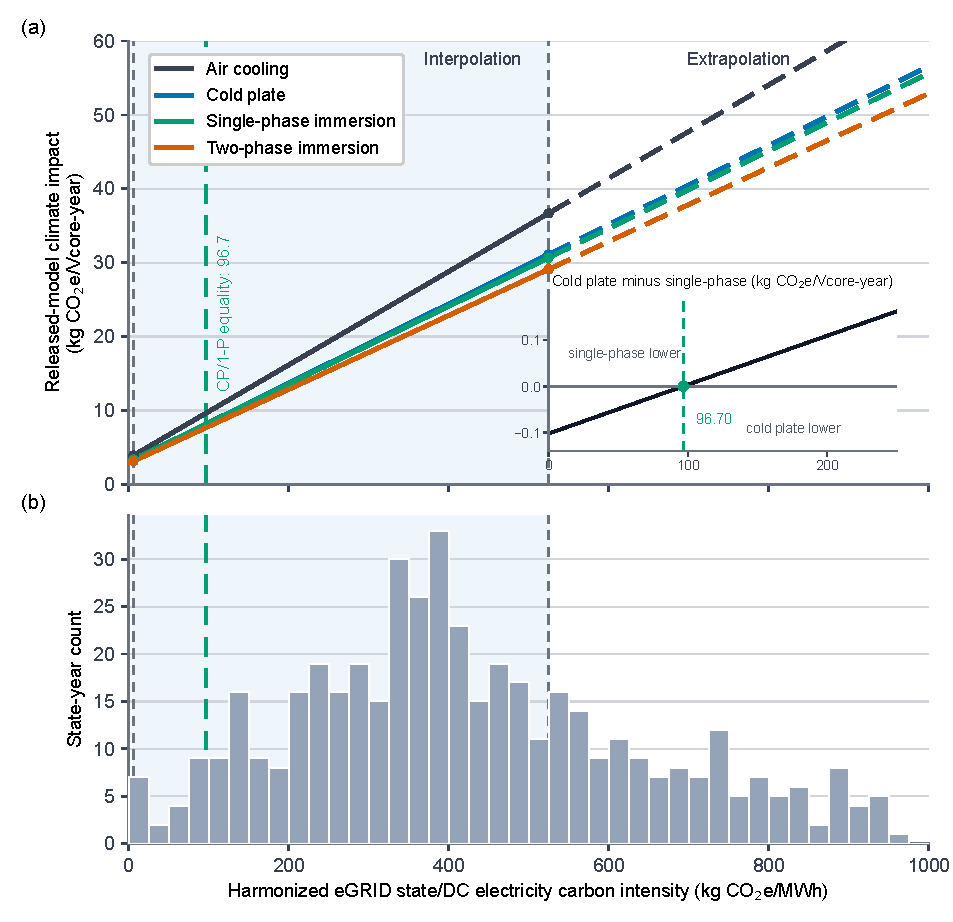
\includegraphics[width=0.78\linewidth]{figure2_released_response_context.pdf}
\caption{Released-model GHG response and eGRID electricity context. In (a), solid lines connect the two released Microsoft/WSP electricity anchors for air cooling, cold plate, single-phase immersion, and two-phase immersion. Dashed segments extend the same numerical relationships beyond those anchors. The green dashed line marks the cold-plate/single-phase equality. Across the released anchor range the cold-plate and single-phase lines differ by at most 0.45 kg \cotwoe{}/Vcore-year, under 1.5\% of either value, so their crossing cannot be resolved on the main axes. The inset plots the difference between them and places the equality at 96.70 kg \cotwoe{}/MWh. In (b), the histogram shows 459 AR5-GWP100 state/DC direct-generation intensities reconstructed from nine eGRID releases. Vertical lines mark the two released electricity anchors and the cold-plate/single-phase equality.}
\label{fig:figure2-released-response-context}
\end{figure}

\subsection{Electricity-system results}
The electricity-system analyses answer two related questions. The eGRID reconstruction tracks how direct generation emissions have changed over time. The Federal LCA Commons calculation quantifies the broader linked electricity system available in a current national and regional inventory.

The common-basis U.S. generation factor declined from 517.731 kg \cotwoe{}/MWh in 2012 to 349.667 kg \cotwoe{}/MWh in 2023, a 32.462\% reduction. The trajectory was not monotonic. The factor rose from 373.097 in 2020 to 388.699 in 2021 before declining. Reconstructing every year with AR5 GWP100 changed the provider-published national rate by no more than 0.248 kg \cotwoe{}/MWh, in 2012. The direct \cotwo{}-only rate was 348.000 kg/MWh in 2023. The long-run decline is therefore not an artifact of eGRID's transition from SAR to AR4 and AR5.

The 50-state-plus-DC reconstruction matched the official national result through 2018. From 2019 onward it was 0.32--0.43\% lower because the dataset covered 99.55--99.58\% of the provider U.S. generation after excluding Puerto Rico. Figure 3 places all 459 harmonized state/DC generation rates from nine eGRID releases on a common kg \cotwoe{}/MWh axis, overlays the reported provider U.S. aggregate trajectory as an orange polyline, and identifies points below the 96.704 kg \cotwoe{}/MWh cold-plate/single-phase crossover in blue. The provider aggregate was retained for the national series and was not fitted to the state/DC points. Across the full dataset, 137 of 459 numerical rates lay outside the two released cooling anchors, so 29.85\% of the transfers were extrapolations. The lowest 2023 direct rate was 23.695 kg \cotwoe{}/MWh, which leaves an exact numerical clearance of 73.009 kg \cotwoe{}/MWh to the cold-plate/single-phase crossover. That clearance is the distance between two values on one axis and is not an estimate of the omitted upstream burden.

\begin{figure}
\centering
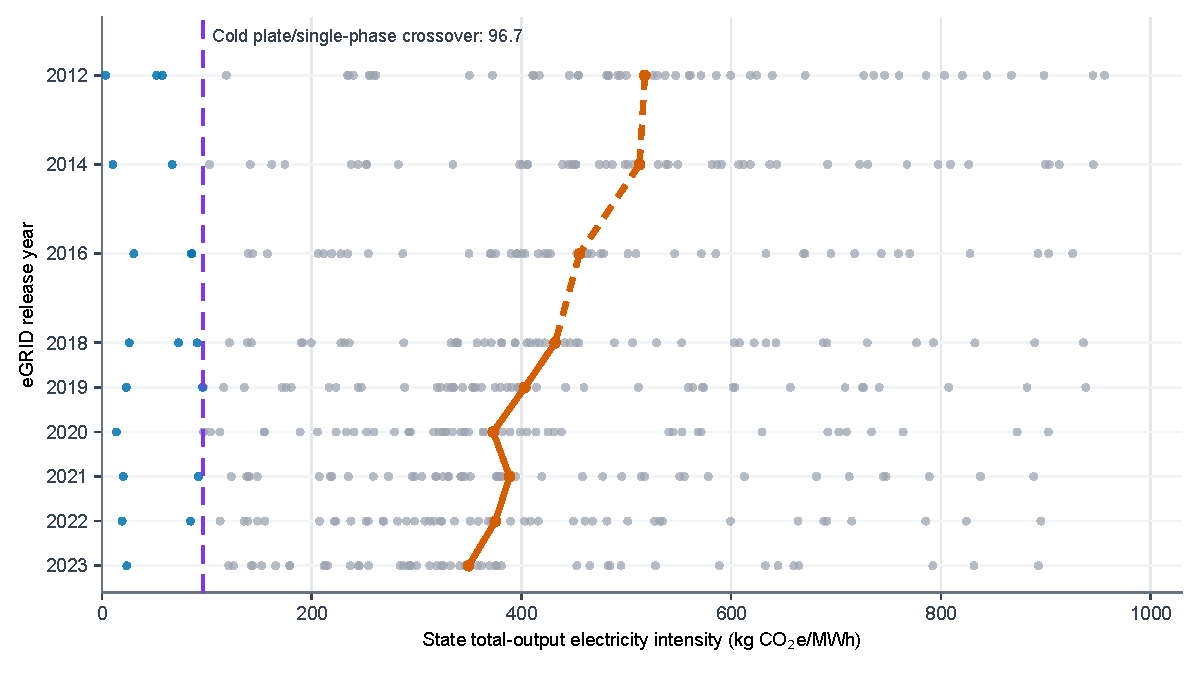
\includegraphics[width=0.98\linewidth]{figure6_historical_grid_transition.pdf}
\caption{Harmonized AR5-GWP100 eGRID state/DC direct-generation rates for nine releases. Electricity intensity is plotted on the horizontal axis in kg \cotwoe{}/MWh. The orange polyline connects the reported provider U.S. aggregate for each year. Blue points lie below the released-workbook numerical cold-plate/single-phase crossover.}
\label{fig:figure6-historical-grid-transition}
\end{figure}

Figure 4 compares the partial linked-system GHG intensity of 10 FERC-region consumption systems and the national system on a delivered-electricity basis. Each bar separates generation-process impacts from other linked upstream and infrastructure impacts, while the two dashed lines locate the 96.704 and 524.893 kg \cotwoe{}/MWh released numerical anchors.

The 71 non-residual Federal LCA Commons systems ranged from 0.921 to 987.844 kg \cotwoe{}/MWh. The national linked-system factor was 422.931 kg \cotwoe{}/MWh. It comprised 369.848 from electricity-generation processes and 53.084 from other linked upstream and infrastructure processes. It exceeded the 2023 national eGRID direct-generation rate by 73.264 kg \cotwoe{}/MWh, although the difference also contains consumption-mix, delivery-loss, flow-coverage, and boundary effects and is not an isolated upstream correction.

All 10 FERC-region systems exceeded the 96.704 kg \cotwoe{}/MWh released-workbook numerical cold-plate/single-phase crossover. Their factors ranged from 238.897 kg \cotwoe{}/MWh for NYISO to 557.110 kg \cotwoe{}/MWh for MISO. Ten of 60 balancing-authority systems fell below the crossover, and 15 of all 71 systems exceeded the released high anchor of 524.893 kg \cotwoe{}/MWh. The numerical cooling screen placed two-phase first in all 71 systems, but this is not a common-method comparative LCA because the cooling foreground method remains unresolved.

The national result converged in five fixed-point iterations with a balance residual of zero at the reporting precision, using 582 processes and 1,174 links. It also contained 287 unlinked technosphere exchanges across 47 processes, including fuels, construction materials, chemicals, and reclaimed water. Their upstream burdens were zero in the linked calculation and were not bounded. The factor is more complete than eGRID direct emissions but still a partial linked-system result.

The national residual-consumption system was 455.350 kg \cotwoe{}/MWh, comprising 399.934 from generation processes and 55.417 from other linked processes. It was 7.67\% above the ordinary consumption-system result. This difference is an electricity-accounting sensitivity, not an uncertainty interval, and the two accounting products were not mixed within any cooling screen.

\begin{figure}
\centering
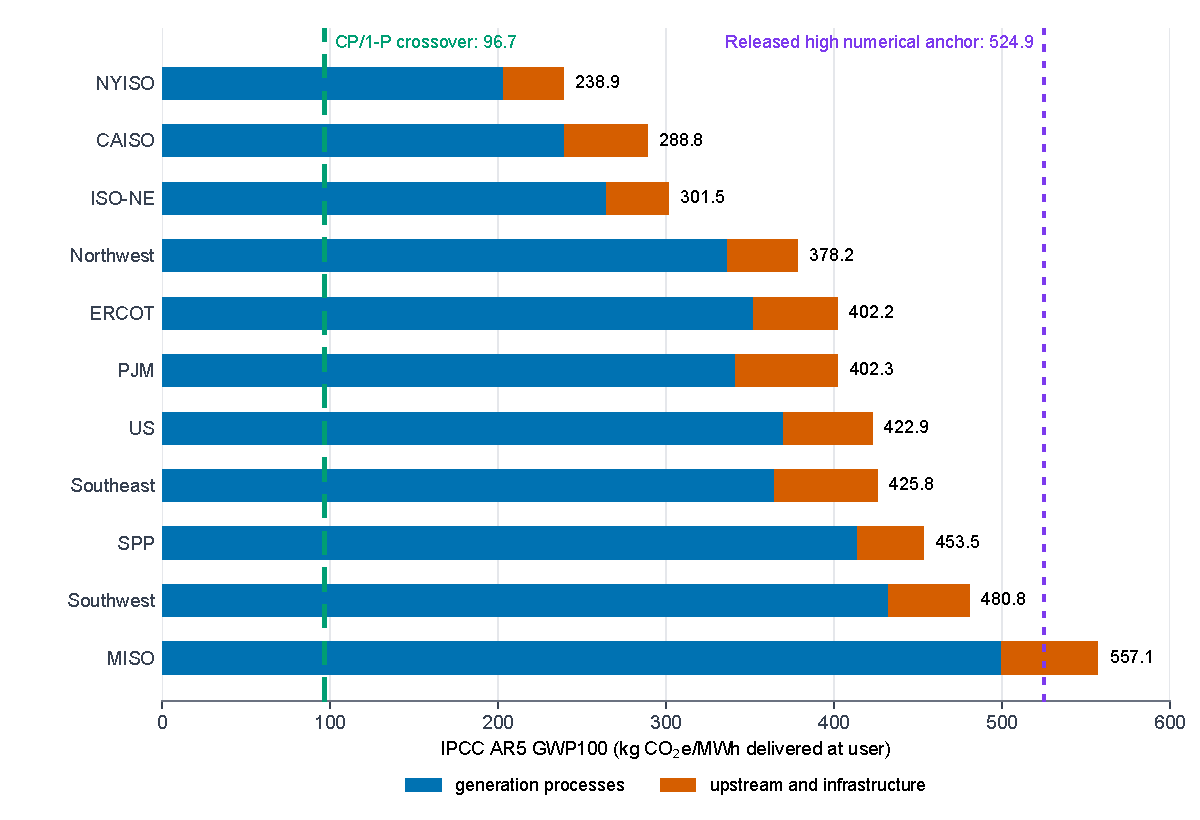
\includegraphics[width=0.98\linewidth]{figure10_lifecycle_electricity.pdf}
\caption{Calculated partial linked-system electricity factors for 10 FERC regions and the United States from the 2023 Federal LCA Commons electricity consumption systems using the IPCC AR5-GWP100 method. The horizontal axis reports kg \cotwoe{}/MWh delivered at the user. Bars separate generation-process impacts from other linked upstream and infrastructure impacts. The green dashed line marks the 96.704 kg \cotwoe{}/MWh released numerical crossover. The purple dashed line marks the 524.893 kg \cotwoe{}/MWh released high numerical anchor. The cooling ranks that these factors support remain numerical screens.}
\label{fig:figure10-lifecycle-electricity}
\end{figure}

\subsection{Rank robustness}
Fig. 5a and Fig. 5b report the same critical half-width $h$. Fig. 5a changes the active assumption block at the national lifecycle-electricity context. Fig. 5b holds all four blocks active at the same $h$ and plots the resulting threshold against lifecycle electricity intensity for 60 balancing authorities, 10 FERC regions, and the national system.

At the national lifecycle factor, the numerical two-phase first rank could not be reversed by a shared grid-factor change within the tested nonnegative range through a 99.999\% half-width. With technology-specific variation, reversal occurred at 2.994\% for use phase, 22.154\% for embodied burden, and 2.637\% for service equivalence. When all four blocks used the same half-width, the first reversal occurred at 1.318\%, against single-phase.

Across all 71 electricity contexts, the all-block critical half-width ranged from 1.123\% at PUD No. 1 of Douglas County to 1.479\% at Duke Energy Progress West. At the lowest-carbon system, the critical competitor was cold plate. At that point, the embodied-only and service-only thresholds were 2.291\% and 2.246\%, while use-phase and shared-grid changes did not reverse rank through 99.999\%. The ranking is numerically fragile even though it survives every unperturbed electricity factor.

This equalized analysis reverses one conclusion from the earlier triangular stress design. Embodied variation had appeared to cause the largest rank loss because its assigned half-width was 10 times those of use phase and service. At equal widths, embodied burden has the largest national one-block tolerance, whereas service equivalence and use phase are limiting. The earlier stress frequencies and their dependence/convergence diagnostics remain in the Supplementary Information as evidence about the chosen design, not the technologies.

The one-sided functional-unit diagnostic gives a complementary threshold. Across 2023 direct-rate contexts, a 5.24--6.04\% adverse correction to two-phase impact per equivalent useful computation would erase its numerical first rank. This is a break-even requirement for future measurements, not an observed performance difference.

\begin{figure}
\centering
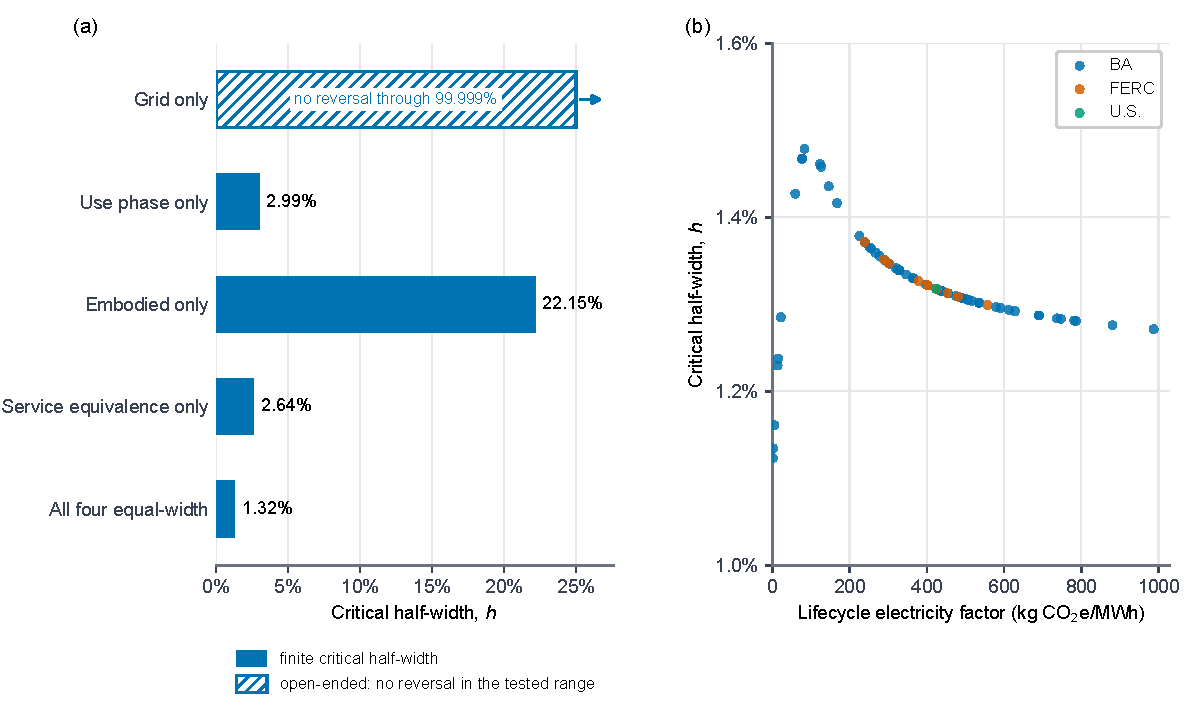
\includegraphics[width=0.98\linewidth]{figure11_standardized_robustness.pdf}
\caption{Deterministic rank-robustness certificates. Both axes report the critical relative half-width $h$, defined as the smallest symmetric relative half-width that permits reversal of the nominal numerical first rank. In (a), the active assumption block changes at the national lifecycle-electricity context. Filled bars report a finite threshold. The hatched open-ended bar marks the shared grid-only set, for which no reversal occurs anywhere in the tested nonnegative range through a 99.999\% half-width. Its drawn length is the axis limit and carries no numerical value. In (b), all four blocks vary at the same $h$, and the threshold is plotted against partial linked-system electricity intensity for 60 balancing authorities, 10 FERC regions, and the national system. Colors in (b) identify the electricity-context level.}
\label{fig:figure11-standardized-robustness}
\end{figure}

\subsection{Foreground evidence priorities}
The published comparison lacks the facility-specific foreground evidence needed to translate a cooling rank into a procurement decision. Server product footprints and construction-material factors indicate the size of that unresolved evidence need, while the contribution-and-pedigree analysis prioritizes the next measurements.

The Boavizta product entries illustrate the scale of missing server-inventory information. Of 55 \texttt{Datacenter/Server} candidates, 48 eligible entries spanned 465--2,503 kg \cotwoe{}/server for manufacturing, a 5.38-fold range. Annualized values spanned 116--626 kg \cotwoe{}/server-year. Scaling the released server-related contributions across the empirical 0.38--2.06-fold annualized envelope retained the deterministic two-phase first rank. The stress test does not model architecture-specific server count, configuration, throughput, or lifetime.

The selected ÖKOBAUDAT high-scrap electric-arc-furnace galvanized-steel factor had 59.9\% lower A1--A3 GHG, 47.9\% lower nonrenewable primary energy, and 52.0\% lower freshwater use per kilogram than the selected low-scrap blast-furnace-route factor. The selected CEM III cement factor had 49.8\% lower GHG, 12.1\% lower nonrenewable primary energy, and 23.5\% lower freshwater use than CEM II/A. These differences identify procurement levers. Their facility effect remains unknown until each architecture has a reviewed bill of quantities.

Under the base contribution-times-weakness index, use phase was the highest priority, followed by storage, networking, and compute-server evidence. Across the nine alternative exponent combinations, use phase ranked first in eight and in the top three in eight. Networking ranked first once, storage remained in the top three in all nine, and compute was in the top three in four. The rank of use phase ranged from first to fourth.

The priority sensitivity changes the interpretation of the pedigree result. The priority sensitivity supports a near-term measurement sequence---hourly IT and cooling electricity, then server inventories and functional performance---but not a unique value of information. A formal acquisition decision requires empirical parameter distributions, correlations, measurement cost, and the loss associated with a wrong architecture choice \cite{ref34}.

\section{Discussion}
\subsection{Comparative claim boundaries}
The released comparison and each unperturbed electricity screen place two-phase immersion first. Three evidence gaps limit the use of that order in a facility decision. The released electricity endpoints have an unresolved climate-method identity, the cooling foreground cannot be recalculated under the same AR5 method as the electricity inventories, and useful computation has not been measured across the four architectures. The resulting rank is therefore a reproduced numerical outcome whose physical basis remains incomplete.

The 96.704 kg \cotwoe{}/MWh cold-plate/single-phase crossover identifies where two released numerical lines intersect. The numerical crossover is not an environmental threshold for a real site. Similarly, the 71 electricity systems explore variation in one background input and do not supply 71 observations of cooling performance. A facility assessment requires the numerical result together with a stated functional unit, impact method, system boundary, cutoff treatment, robustness definition, and claim scope.

\subsection{Electricity-system boundaries}
The eGRID reconstruction shows that the 32.46\% historical national decline is robust to changing GWP conventions. The Federal LCA Commons calculation then replaces an arbitrary additive boundary allowance with a provider-linked consumption model. At the national point, linked upstream and infrastructure processes add 53.084 kg \cotwoe{}/MWh beyond generation processes, and the total is 73.264 kg \cotwoe{}/MWh above the eGRID national rate. All FERC regions lie above the numerical cold-plate/single-phase crossover.

Provider-linked consumption modeling improves boundary traceability but does not complete harmonization because the difference between the two national factors also reflects delivery losses, consumption versus generation geography, and elementary-flow coverage. More importantly, 287 unlinked technosphere exchanges still carry zero upstream burden. A complete calculation requires those providers to be linked or their omitted impacts to be bounded and independently reproduced. Even then, electricity cannot repair the unresolved cooling-foreground LCIA method. Location- and market-based cases must also remain consistent throughout the product system \cite{ref22,ref23}. The 7.67\% national difference between ordinary and residual consumption mixes shows that the accounting choice is consequential even before the cooling foreground is harmonized.

\subsection{Robustness-bound design}
The earlier triangular analysis assigned embodied burden a half-width 10 times the use-phase and service widths. Its conclusion that embodied variation was the largest one-block source of rank loss therefore combined model sensitivity with an arbitrary range choice. The equal-width certificate separates those effects. At the national lifecycle factor, embodied burden can vary by 22.15\% before a worst-case one-block reversal, whereas service equivalence and use phase require only 2.64\% and 2.99\%. The all-block threshold of 1.32\% describes the radius of a specified box in which a shared grid multiplier and adverse technology-specific foreground multipliers can reverse the numerical first rank. Any empirical uncertainty model can be evaluated against the same bound structure, although a probability of rank would require measured marginal distributions and correlations \cite{ref30}. Functional equivalence and use-phase demand are thus the first evidence gaps to close, followed by bills of quantities and material inventories needed for a common-method lifecycle comparison. The legacy triangular results still show that dependence assumptions matter, but they do not rank the real-world importance of the uncertainty blocks.

\subsection{Functional equivalence}
Vcore-year is more informative than facility area or rack count, but it is still a proxy. Equivalent useful computation depends on workload, accelerator utilization, memory and network constraints, throttling, overclocking, availability, and quality of service. The one-sided 5.50\% median threshold and the symmetric 2.64\% national service bound are break-even requirements, not measured penalties. They define the approximate resolution required of a comparative experiment. ITU-T L.1410 similarly requires an explicit functional unit and comparative baseline for ICT services \cite{ref18}.

A shared protocol should collect several forms of evidence for every architecture. It should measure i) completed workload or benchmark output, ii) IT and cooling power, and iii) inlet and component temperatures together with flow and pressure drop. It should also measure iv) fan, pump, cooling distribution unit, and heat-rejection power, v) onsite water use and failure or maintenance events, and vi) uncertainty and calibration information over the same load-weather domain. Server count, configuration, and replacement must accompany the performance data. A thermal result without useful computation cannot close the LCA functional unit. A product carbon footprint without architecture quantity cannot close the embodied inventory.

\subsection{Grid decarbonization and evidence priorities}
National grid decarbonization simultaneously lowers every electricity-dependent cooling result, contracts the absolute value of operational efficiency, and increases the fraction supplied by embodied terms. The absolute modeled two-phase-versus-air benefit fell 29.45\% between the 2012 and 2023 generation conditions, a change that percentage savings alone do not reveal. This shift explains why the Boavizta and ÖKOBAUDAT datasets matter even though they were not inserted into architecture totals. The 5.38-fold server manufacturing range is larger than many cooling differences, yet heterogeneous PCFs cannot serve as an uncertainty distribution for interchangeable servers. The approximately 50--60\% material-route GHG levers are large per kilogram, although kilograms by architecture are unavailable. A facility-specific analysis needs a linked foreground dataset that combines useful computation, server configuration and lifetime, cooling bill of quantities, material route, and measured operation under one functional unit.

\subsection{Relationship to LCA software}
OpenDC-LCA supplements openLCA, Brightway, Temporalis, premise, and bw\_timex, which provide process-network calculation, database management, prospective backgrounds, or time-explicit LCA \cite{ref27,ref28,ref29,ref37,ref38}. Its assessment layer tests comparison compatibility before calculation by linking functional equivalence to useful computation, representing documented cooling, replacement, and fluid information when those data are available, and separating lifecycle electricity from direct-generation, market-based, and marginal signals. The package also retains source and transformation provenance. Its automated metadata validator blocks declared comparisons with incompatible methods, boundaries, or source mappings.

The metadata validator is deliberately narrower than a scientific review because it trusts the metadata supplied by the user and cannot determine whether a performance map is representative, a distribution is empirical, or an external review occurred. Its role is to catch machine-detectable incompatibilities before calculation, not to authorize a public environmental claim.

The comparison-audit role differs from recent data center performance and architecture models. AlphaDataCenterCooling provides operational validation of a cooling plant \cite{ref17}, while d'Orgeval et al. compare full data center architectures and, for a subset, normalize by computational performance \cite{ref16}. OpenDC-LCA tests whether published secondary LCA results retain their meaning when moved across electricity datasets and claim contexts. OpenDC-LCA does not duplicate either primary modeling capability.

USLCI and GLAD hydrogen archives were exchange-tested but were not used as numerical evidence. Backup power is a relevant future application, yet a hydrogen dataset becomes numerical evidence only after technology, electricity source, compression/storage, allocation, geography, and LCIA method are linked to a declared product system.

\subsection{Operational validation}
Facility-specific validation requires a common service measure and time-aligned measurements of IT, electrical, and cooling operation. The released comparison also requires traceable electricity factors, architecture-specific bills of quantities, and a resolved climate-impact method before its results can be updated as a common-method LCA. A preliminary university high-performance-computing site characterization illustrates this boundary. The site combines dedicated IT and liquid-cooling paths with raised-floor CRAC cooling shared by several institutional users. Available information identifies equipment and shared infrastructure, whereas operational time series are unavailable. It therefore provides no energy, cooling-performance, PUE, or environmental result in this paper.

The repository includes a measurement protocol for a future shared-infrastructure assessment. It identifies the meter locations, allocation information, thermal measurements, workload information, and calibration metadata needed to calculate a dedicated-support ratio or a facility PUE. The protocol also retains the electrical hierarchy and liquid-loop measurement points required to interpret a cooling result \cite{ref53,ref54,ref55,ref56}. The released arithmetic and the national direct-generation trend are the two findings supported independently by the available sources. Cooling crossovers, first ranks, and response coefficients remain conditional numerical results until the required method, inventory, service, and operating evidence becomes available.

\subsection{Evidence requirements and limitations}
The present analysis uses secondary sources and released numerical materials. It does not recreate proprietary background inventories, confidential bills of quantities, the full virtual-core model, or measured hyperscale operation. Equation (8) retains an unresolved climate-method identity, and the Federal LCA Commons factors contain 287 national unlinked technosphere exchanges. The custom solver awaits independent reproduction in openLCA or Brightway. The additive allowance, triangular marginals, and copula dependence cases are specified diagnostic cases. Their convergence check quantifies numerical sampling precision within those cases and does not constrain uncertainty in the input ranges, dependence structure, cutoff treatment, or cooling foreground. The climate analysis reports greenhouse-gas emissions only and provides no common-method comparison of primary energy, water scarcity, toxicity, or resource use. Boavizta entries use heterogeneous products and methods, while ÖKOBAUDAT supplies German generic A1--A3 factors. The TMY and synthetic performance examples test software pathways, and the USGS file supplies watershed geometry. These sources cannot supply measured cooling performance, a facility water balance, or AWARE characterization. The available evidence therefore supports a case-study evaluation of whether the released cooling comparison can be applied to a new facility. A public claim of environmental superiority would require common-method inventories, reviewed primary performance and useful-computation data, architecture bills of quantities, water-scarcity characterization, empirically supported joint uncertainty, and an external critical review.

The OCP documents provide a practical template for the missing foreground information. A future vendor or facility inventory should identify the manufacturer, part number, quantity, functional unit, lifecycle modules, calculation method, background database, geography, reference year, verification status, source location, service life, and replacement rule \cite{ref51}. Where water is evaluated, on-site consumption and electricity-supply-chain water should remain separate, and a water-use-effectiveness value should retain its IT-energy denominator and site boundary \cite{ref52}. The repository supplies a companion template for this information. Independent reproduction of the Federal electricity systems is the next calculation step. The national, low, and high systems should be reproduced in openLCA or Brightway using the same JSON-LD product systems and IPCC method. The comparison should report the software version, target amount, process count, link count, characterized total, and unlinked-exchange count. Any difference should be traced to unit conversion, provider resolution, characterization, or cutoff treatment. The partial linked-system factors remain screening inputs until this check and a quantitative cutoff bound are available.

\section{Conclusions}
The Microsoft/WSP case study shows the evidence needed before a published cooling comparison can guide a data center decision. Arithmetic reconstruction matched all 24 released totals. The available electricity information did not resolve the stated AR5 GWP100 basis, so the published ranks remain reproducible numerical outcomes instead of verified common-method comparative LCA results. Nine eGRID releases showed a 32.46\% decline in the U.S. national direct-generation factor between 2012 and 2023. The national Federal LCA Commons calculation yielded 422.93 kg \cotwoe{}/MWh and retained 287 unlinked technosphere exchanges. These electricity results give transparent screening context, while their boundaries and remaining cutoffs preclude direct substitution into the cooling comparison. The nominal first rank reversed when all declared assumption blocks moved adversely by an equal half-width of 1.32\%. This worst-case bound identifies comparable computing service and time-aligned use-phase demand as immediate evidence needs. Architecture-resolved equipment inventories are the next requirement for a facility-specific life cycle assessment. The software applies declared functional-unit, boundary, electricity-accounting, climate-method, and source-mapping requirements before calculation. Physical performance, source accuracy, and review quality remain outside automated validation and require primary evidence and independent review.

\section{Data and code availability}
OpenDC-LCA version 1.1.0 is publicly available at \url{https://github.com/UARK-NED3/OpenDC-LCA} and \url{https://github.com/UARK-NED3/OpenDC-LCA/releases/tag/v1.1.0}. The development revision evaluated here adds the Federal LCA Commons solver, cutoff reporting, equal-width robustness certificates, and comparison-level metadata checks. The code, derived tables, figures, manuscript source, environment specification, and provenance manifest for this revision are deposited in an immutable DOI-bearing archive at \textbf{[DOI PLACEHOLDER]}. Each reported value carries a provenance manifest entry that records the source file hash, the generating module, and the fixed seeds and iteration counts. Provider-native files remain outside Git when redistribution permission is unclear or a large upstream archive has not been reviewed for redistribution. The Microsoft archive, eGRID files, Federal LCA Commons baseline and method, and NOAA data are available from their public providers \cite{ref15,ref40,ref41,ref42,ref45}.

\section{Competing interests}
Braden Stevens and Pengjiang Xiang are full-time employees of Harrison French \& Associates Ltd.

\section{Ethics statement}
The secondary study used public or author-held engineering datasets and did not involve human participants or animals. Research-ethics approval was not required.

\section{Author-contribution and funding confirmation}
A CRediT author-contribution statement, funding statement, acknowledgments, and confirmation of any additional competing interests require all-author approval before submission. They are not inferred in this draft.

\section{Declaration of generative AI and AI-assisted technologies in the manuscript preparation process}
During preparation of this work, the authors used OpenAI Codex to support code review, test development, figure-code review, manuscript organization, and language editing. The authors reviewed and edited the resulting material, verified the reported calculations and cited sources, and take full responsibility for the content of the article.

\begin{thebibliography}{99}
\bibitem{ref1} Masanet, E., Shehabi, A., Lei, N., Smith, S. \& Koomey, J. Recalibrating global data center energy-use estimates. \textit{Science} \textbf{367}, 984--986 (2020). \url{https://doi.org/10.1126/science.aba3758}
\bibitem{ref2} International Energy Agency. Data centres and data transmission networks. \url{https://www.iea.org/energy-system/buildings/data-centres-and-data-transmission-networks} (accessed 11 August 2026).
\bibitem{ref3} Khalaj, A. H. \& Halgamuge, S. K. A review on efficient thermal management of air- and liquid-cooled data centers. \textit{Applied Energy} \textbf{205}, 1165--1184 (2017). \url{https://doi.org/10.1016/j.apenergy.2017.08.037}
\bibitem{ref4} Alkrush, A. A., Salem, M. S., Abdelrehim, O. \& Hegazi, A. A. Data centers cooling: a critical review of techniques, challenges, and energy saving solutions. \textit{International Journal of Refrigeration} \textbf{160}, 246--262 (2024). \url{https://doi.org/10.1016/j.ijrefrig.2024.02.007}
\bibitem{ref5} Kanbur, B. B., Wu, C., Fan, S. \& Duan, F. Two-phase liquid-immersion data center cooling system: experimental performance and thermoeconomic analysis. \textit{International Journal of Refrigeration} \textbf{118}, 290--301 (2020). \url{https://doi.org/10.1016/j.ijrefrig.2020.05.026}
\bibitem{ref6} Kanbur, B. B., Wu, C., Fan, S. \& Duan, F. System-level experimental investigations of direct immersion cooling data center units with thermodynamic and thermoeconomic assessments. \textit{Energy} \textbf{217}, 119373 (2021). \url{https://doi.org/10.1016/j.energy.2020.119373}
\bibitem{ref7} Huang, Y., Liu, B., Xu, S., Bao, C., Zhong, Y. \& Zhang, C. Experimental study on immersion liquid cooling performance of high-power data center servers. \textit{Energy} \textbf{297}, 131195 (2024). \url{https://doi.org/10.1016/j.energy.2024.131195}
\bibitem{ref8} Wu, X. et al. Investigations on heat dissipation performance and overall characteristics of two-phase liquid immersion cooling systems for data center. \textit{International Journal of Heat and Mass Transfer} \textbf{239}, 126575 (2025). \url{https://doi.org/10.1016/j.ijheatmasstransfer.2024.126575}
\bibitem{ref9} Whitehead, B., Andrews, D., Shah, A. \& Maidment, G. Assessing the environmental impact of data centres. Part 1: background, energy use and metrics. \textit{Building and Environment} \textbf{82}, 151--159 (2014). \url{https://doi.org/10.1016/j.buildenv.2014.08.021}
\bibitem{ref10} Siddik, M. A. B., Shehabi, A. \& Marston, L. The environmental footprint of data centers in the United States. \textit{Environmental Research Letters} \textbf{16}, 064017 (2021). \url{https://doi.org/10.1088/1748-9326/abfba1}
\bibitem{ref11} Ristic, B., Madani, K. \& Makuch, Z. The water footprint of data centers. \textit{Sustainability} \textbf{7}, 11260--11284 (2015). \url{https://doi.org/10.3390/su70811260}
\bibitem{ref12} Isler-Kaya, A. \& Karaosmanoglu, F. Life cycle assessment of a climate-friendly data center cooling device. \textit{Energy and Buildings} \textbf{288}, 113006 (2023). \url{https://doi.org/10.1016/j.enbuild.2023.113006}
\bibitem{ref13} Wenzel, P. M. \& Radgen, P. Extending effectiveness to efficiency: comparing energy and environmental assessment methods for a wet cooling tower. \textit{Journal of Industrial Ecology} \textbf{27}, 693--706 (2023). \url{https://doi.org/10.1111/jiec.13396}
\bibitem{ref14} Alissa, H. et al. Using life cycle assessment to drive innovation for sustainable cool clouds. \textit{Nature} \textbf{641}, 331--338 (2025). \url{https://doi.org/10.1038/s41586-025-08832-3}
\bibitem{ref15} Alissa, H. et al. Data and model archive for ``Using life cycle assessment to drive innovation for sustainable cool clouds.'' Zenodo record 14268168 (2024). \url{https://doi.org/10.5281/zenodo.14268168}
\bibitem{ref16} d'Orgeval, A., Sheehan, S., Avenas, Q., Assoumou, E. \& Sessa, V. Generative AI impact assessment through a life cycle analysis of multiple data center typologies. \textit{Applied Energy} \textbf{406}, 127288 (2026). \url{https://doi.org/10.1016/j.apenergy.2025.127288}
\bibitem{ref17} Wu, S., Zheng, W., Wang, Z., Chen, G., Yang, P., Yue, S., Li, D. \& Wu, Y. AlphaDataCenterCooling: A new computational model for data center cooling system evaluation. \textit{Applied Energy} \textbf{380}, 125100 (2025). \url{https://doi.org/10.1016/j.apenergy.2024.125100}
\bibitem{ref18} International Telecommunication Union. ITU-T Recommendation L.1410: Methodology for environmental life cycle assessments of information and communication technology goods, networks and services (2024). \url{https://handle.itu.int/11.1002/1000/16010}
\bibitem{ref19} Zhang, M., Carbajales-Dale, M., Ma, X., Guo, L. \& Fan, C. Cleaner grid or smarter cooling? Environmental impact trade-offs of a data center using the life cycle assessment method. \textit{Cleaner Energy Systems} \textbf{12}, 100223 (2025). \url{https://doi.org/10.1016/j.cles.2025.100223}
\bibitem{ref20} Boyd, S. B., Horvath, A. \& Dornfeld, D. Life-cycle assessment of computational logic produced from 1995 through 2010. \textit{Environmental Science \& Technology} \textbf{47}, 2947--2954 (2013). \url{https://doi.org/10.1021/es303012r}
\bibitem{ref21} Malmodin, J. \& Lundén, D. The energy and carbon footprint of the global ICT and E\&M sectors 2010--2015. \textit{Sustainability} \textbf{10}, 3027 (2018). \url{https://doi.org/10.3390/su10093027}
\bibitem{ref22} Holzapfel, P., Bach, V. \& Finkbeiner, M. Electricity accounting in life cycle assessment: the challenge of double counting. \textit{International Journal of Life Cycle Assessment} \textbf{28}, 771--787 (2023). \url{https://doi.org/10.1007/s11367-023-02158-w}
\bibitem{ref23} Holzapfel, P., Bunsen, J., Schmidt-Sierra, I., Bach, V. \& Finkbeiner, M. Replacing location-based electricity consumption with market-based residual mixes in background data to avoid possible double counting. \textit{International Journal of Life Cycle Assessment} \textbf{29}, 1279--1289 (2024). \url{https://doi.org/10.1007/s11367-024-02294-x}
\bibitem{ref24} Dandres, T., Farrahi Moghaddam, R., Nguyen, K. K., Lemieux, Y., Samson, R. \& Cheriet, M. Consideration of marginal electricity in real-time minimization of distributed data centre emissions. \textit{Journal of Cleaner Production} \textbf{143}, 116--124 (2017). \url{https://doi.org/10.1016/j.jclepro.2016.12.143}
\bibitem{ref25} Sohn, J., Kalbar, P., Goldstein, B. \& Birkved, M. Defining temporally dynamic life cycle assessment: a review. \textit{Integrated Environmental Assessment and Management} \textbf{16}, 314--323 (2020). \url{https://doi.org/10.1002/ieam.4235}
\bibitem{ref26} Beloin-Saint-Pierre, D. et al. Addressing temporal considerations in life cycle assessment. \textit{Science of the Total Environment} \textbf{743}, 140700 (2020). \url{https://doi.org/10.1016/j.scitotenv.2020.140700}
\bibitem{ref27} Cardellini, G., Mutel, C. L., Vial, E. \& Muys, B. Temporalis, a generic method and tool for dynamic life cycle assessment. \textit{Science of the Total Environment} \textbf{645}, 585--595 (2018). \url{https://doi.org/10.1016/j.scitotenv.2018.07.044}
\bibitem{ref28} Müller, A. et al. Time-explicit life cycle assessment: a flexible framework for coherent consideration of temporal dynamics. \textit{International Journal of Life Cycle Assessment} (2025). \url{https://doi.org/10.1007/s11367-025-02539-3}
\bibitem{ref29} Diepers, T., Müller, A. \& Jakobs, A. bw\_timex: a Python package for time-explicit life cycle assessment. \textit{Journal of Open Source Software} \textbf{11}, 9621 (2026). \url{https://doi.org/10.21105/joss.09621}
\bibitem{ref30} Groen, E. A. \& Heijungs, R. Ignoring correlation in uncertainty and sensitivity analysis in life cycle assessment: what is the risk? \textit{Environmental Impact Assessment Review} \textbf{62}, 98--109 (2017). \url{https://doi.org/10.1016/j.eiar.2016.10.006}
\bibitem{ref31} Michiels, F. \& Geeraerd, A. How to decide and visualize whether uncertainty or variability is dominating in life cycle assessment results: a systematic review. \textit{Environmental Modelling \& Software} \textbf{133}, 104841 (2020). \url{https://doi.org/10.1016/j.envsoft.2020.104841}
\bibitem{ref32} Lloyd, S. M. \& Ries, R. Characterizing, propagating, and analyzing uncertainty in life-cycle assessment: a survey of quantitative approaches. \textit{Journal of Industrial Ecology} \textbf{11}, 161--179 (2007). \url{https://doi.org/10.1162/jiec.2007.1136}
\bibitem{ref33} Edelen, A. \& Ingwersen, W. Guidance on Data Quality Assessment for Life Cycle Inventory Data. U.S. EPA, EPA/600/R-16/096 (2016). \url{https://cfpub.epa.gov/si/si_public_record_report.cfm?Lab=NRMRL&dirEntryId=321834}
\bibitem{ref34} Marchese, D. C., Bates, M. E., Keisler, J. M., Alcaraz, M. L., Linkov, I. \& Olivetti, E. A. Value of information analysis for life cycle assessment: uncertain emissions in green manufacturing of electronic tablets. \textit{Journal of Cleaner Production} \textbf{197}, 1540--1545 (2018). \url{https://doi.org/10.1016/j.jclepro.2018.06.113}
\bibitem{ref35} International Organization for Standardization. ISO 14040:2006, Environmental management - Life cycle assessment - Principles and framework; and ISO 14044:2006, Environmental management - Life cycle assessment - Requirements and guidelines. \url{https://www.iso.org/committee/54854/x/catalogue/;} \url{https://www.iso.org/standard/38498.html} (accessed 11 August 2026).
\bibitem{ref36} International Organization for Standardization. ISO 14071:2024, Environmental management - Life cycle assessment - Critical review processes and reviewer competencies (2024). \url{https://www.iso.org/standard/82464.html} (accessed 11 August 2026).
\bibitem{ref37} GreenDelta. openLCA: open source life cycle assessment software. \url{https://www.openlca.org/} (accessed 11 August 2026).
\bibitem{ref38} Mutel, C. Brightway: an open source framework for life cycle assessment. \textit{Journal of Open Source Software} \textbf{2}, 236 (2017). \url{https://doi.org/10.21105/joss.00236}
\bibitem{ref39} UARK-NED3. OpenDC-LCA version 1.1.0. \url{https://github.com/UARK-NED3/OpenDC-LCA} (accessed 11 August 2026).
\bibitem{ref40} U.S. Environmental Protection Agency. Emissions \& Generation Resource Integrated Database (eGRID), detailed data. \url{https://www.epa.gov/egrid/detailed-data} (accessed 11 August 2026).
\bibitem{ref41} U.S. Environmental Protection Agency. Frequent questions about eGRID: global warming potentials and methodology changes. \url{https://www.epa.gov/egrid/frequent-questions-about-egrid} (accessed 11 August 2026).
\bibitem{ref42} National Energy Technology Laboratory. U.S. Electricity Baseline, 2023 data release, version 03.00.000. Federal LCA Commons (2026). \url{https://www.lcacommons.gov/lca-collaboration/Federal_LCA_Commons/US_electricity_baseline} (accessed 11 August 2026).
\bibitem{ref43} Boavizta. BoaviztAPI data repository. \url{https://github.com/Boavizta/boaviztapi} (accessed 11 August 2026).
\bibitem{ref44} Bundesinstitut für Bau-, Stadt- und Raumforschung. ÖKOBAUDAT 2024-II. \url{https://www.oekobaudat.de/} (accessed 11 August 2026).
\bibitem{ref45} National Centers for Environmental Information. Typical Meteorological Year data. \url{https://www.ncei.noaa.gov/access/typical-meteorological-year/} (accessed 11 August 2026).
\bibitem{ref46} National Renewable Energy Laboratory. U.S. Life Cycle Inventory Database, version 1.2026-06.0. Federal LCA Commons. \url{https://www.lcacommons.gov/} (accessed 11 August 2026).
\bibitem{ref47} United Nations Environment Programme. Global LCA Data Access network. \url{https://www.globallcadataaccess.org/} (accessed 11 August 2026).
\bibitem{ref48} U.S. Geological Survey. Watershed Boundary Dataset. \url{https://www.usgs.gov/national-hydrography/watershed-boundary-dataset} (accessed 11 August 2026).
\bibitem{ref49} Sun, K., Luo, N., Luo, X. \& Hong, T. Prototype energy models for data centers. \textit{Energy and Buildings} \textbf{231}, 110603 (2021). \url{https://doi.org/10.1016/j.enbuild.2020.110603}
\bibitem{ref50} Open Compute Project Foundation. \textit{Guidelines: Life Cycle Assessment, LCA Guidelines for Cloud Providers}. \url{https://www.opencompute.org/documents/lca-sop-in-ocp-document-submission-template-docx-pdf} (accessed 9 September 2026).
\bibitem{ref51} Open Compute Project Foundation \& iMasons Climate Accord. \textit{Embodied Carbon Disclosure Base Specification}, version 1 (July 2025). \url{https://www.opencompute.org/documents/carbon-disclosure-ocp-base-specification-20250730-pdf} (accessed 9 September 2026).
\bibitem{ref52} Open Compute Project Foundation. \textit{Guidelines: Impact of Strategies on Data Center Energy Consumption, Carbon Footprint, and Water Consumption} (March 2026). \url{https://www.opencompute.org/documents/dcf-water-heat-energy-2026march-pdf} (accessed 9 September 2026).
\bibitem{ref53} Sharp, S., Kaneko, M., Chen, M., Shahi, P., Karajgikar, S. \& James, D. \textit{Third Party Integration, Telemetry \& APIs}, version 1.0 (October 2025). Open Compute Project Foundation. \url{https://www.opencompute.org/documents/third-party-integration-telemetry-apis-final-pdf} (accessed 9 September 2026).
\bibitem{ref54} Mitchell, D. \textit{et al.} \textit{Guidelines for Connection of Liquid Cooled Information Technology Equipment to Data Center Facility Systems}, revision 1, version 1.0 (April 2022). Open Compute Project Foundation. \url{https://www.opencompute.org/documents/ocp-acs-connection-guidance-acf-wp-05032022-pdf} (accessed 9 September 2026).
\bibitem{ref55} Mitchell, D. \textit{et al.} \textit{Data Center Liquid Distribution Guidance \& Reference Designs}, revision 1.0 (January 2024). Open Compute Project Foundation. \url{https://www.opencompute.org/documents/ocp-acf-reference-design-guidance-white-paper-r1-pdf} (accessed 9 September 2026).
\bibitem{ref56} Yaroch, K., Cuthbert, J., Miller, D. \& Sivapalan, S. \textit{Guidelines for Using Propylene Glycol-Based Heat Transfer Fluids in Single-Phase Cold Plate-Based Liquid Cooled Racks}. Open Compute Project Foundation. \url{https://www.opencompute.org/contributions} (accessed 9 September 2026).
\end{thebibliography}
\end{document}
